\begin{appendix}

\FloatBarrier
\section{Code repository}
All code used for this project is available at \href{https://github.com/ericludvigs/AST5220_Cosmology_Project}{this Github repository}.
Description of code folders and places to look here.

\FloatBarrier
\section{Milestone I, extra plots}\label{app:milestone_1_extra_plots}

Evolution of some physical quantities in figs. \ref{fig:milestone_1_H_prime_of_x} and \ref{fig:milestone_1_eta_of_x}.

\begin{figure}[h!tb]
\centering
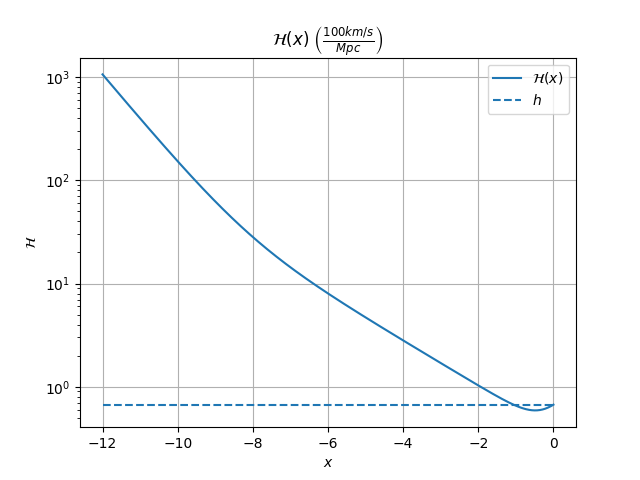
\includegraphics[width=0.4\textwidth]{../Milestone 1/Plots/H_prime_of_x.png}
\caption{Caption}
\label{fig:milestone_1_H_prime_of_x}
\end{figure}

\begin{figure}[h!bt]
\centering
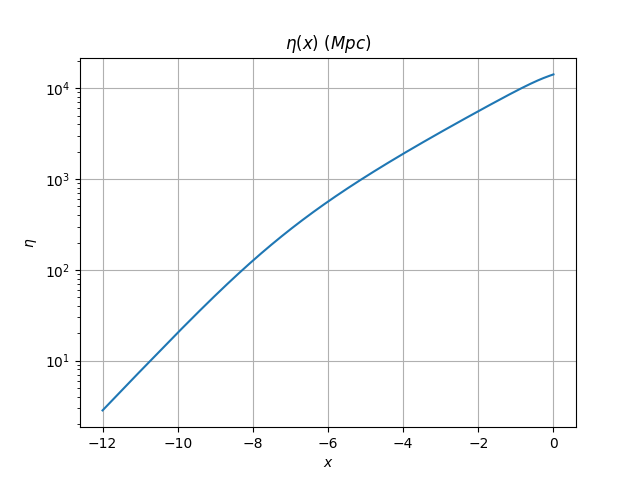
\includegraphics[width=0.4\textwidth]{../Milestone 1/Plots/eta_of_x.png}
\caption{Caption}
\label{fig:milestone_1_eta_of_x}
\end{figure}

Histograms of parameter distribution in fig. \ref{fig:milestone_1_appendix_histograms}.

\begin{figure*}[h!tb]
\centering
    \begin{subfigure}[t!]{0.4\textwidth}
    \centering
    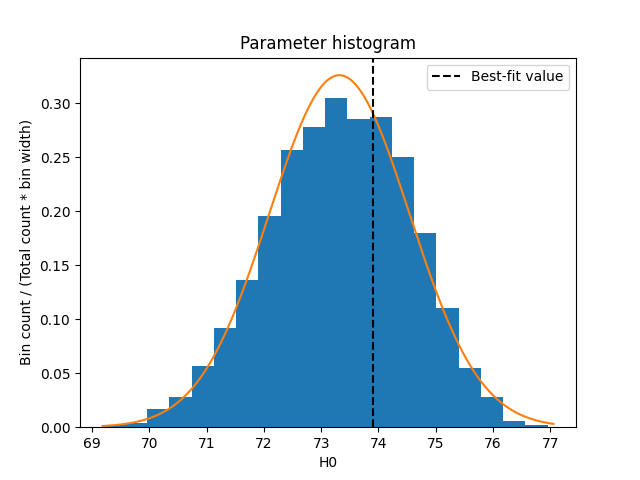
\includegraphics[width=1.0\textwidth]{../Milestone 1/Plots/H0_histogram.png}
    \caption{Caption 1}
    \label{fig:milestone_1_H0_histogram}
    \end{subfigure}
    %\hfill
    \begin{subfigure}[t!]{0.4\textwidth}
    \centering
    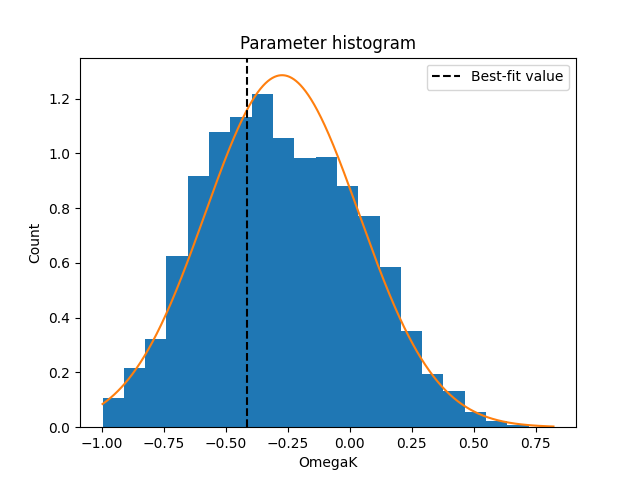
\includegraphics[width=1.0\textwidth]{../Milestone 1/Plots/OmegaK_histogram.png}
    \caption{Caption 2}
    \label{fig:milestone_1_OmegaK_histogram}
    \end{subfigure}
    \hfill
    %\hfill
    \begin{subfigure}[b!]{0.4\textwidth}
    \centering
    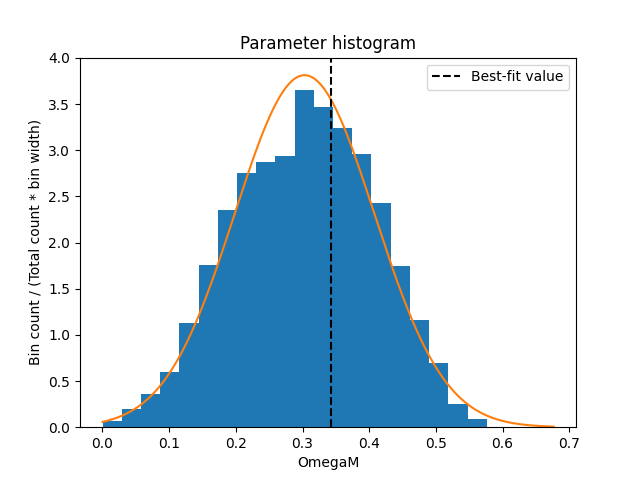
\includegraphics[width=1.0\textwidth]{../Milestone 1/Plots/OmegaM_histogram.png}
    \caption{Caption 3}
    \label{fig:milestone_1_OmegaM_histogram}
    \end{subfigure}
    \begin{subfigure}[b!]{0.4\textwidth}
    \centering
    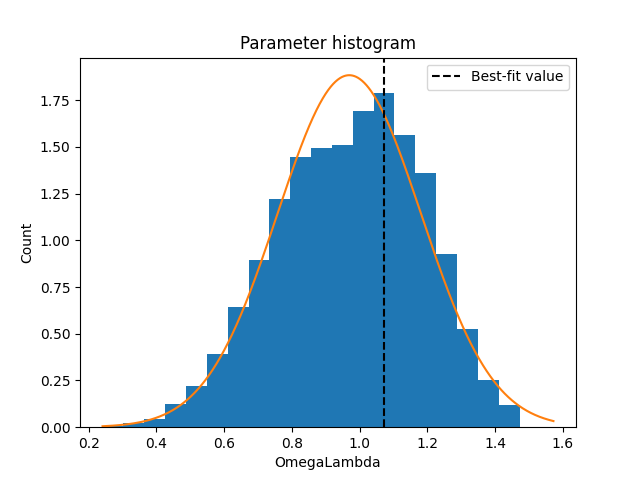
\includegraphics[width=1.0\textwidth]{../Milestone 1/Plots/OmegaLambda_histogram.png}
    \caption{Caption 4}
    \label{fig:milestone_1_OmegaLambda_histogram}
    \end{subfigure}
\caption{Whole figure caption}
\label{fig:milestone_1_appendix_histograms}
\end{figure*}

%\FloatBarrier
\section{Milestone II, extra math}
Definitions to support Peebles equation (\ref{eq:peebles_equation}):

\boxed{
\begin{aligned}\label{eq:peebles_quantities_definition}
C_r(T_b) &= \frac{\Lambda_{2s\rightarrow1s} + \Lambda_{\alpha}}{\Lambda_{2s\rightarrow1s} + \Lambda_{\alpha} + \beta^{(2)}(T_b)}, \,\,{\rm (dimensionless)}\\
H &,  \,\,{\rm (dimension~1/s)}\\
\Lambda_{2s\rightarrow1s} &= 8.227, \,\,{\rm (dimension~1/s)}\\
\Lambda_{\alpha} &= H\frac{(3\epsilon_0)^3}{(8\pi)^2 n_{1s}}, \,\,{\rm (dimension~1/s)}\\
n_{1s} &= (1-X_e)n_H, \,\,{\rm (dimension~1/m^3)}\\
n_H &= (1-Y_p)\frac{3H_0^2\Omega_{b0}}{8\pi G m_H a^3}, \,\,{\rm (dimension~1/m^3)}\\
\beta^{(2)}(T_b) &= \beta(T_b) e^{3\epsilon_0/4T_b}, \,\,{\rm (dimension~1/s)}\\
\beta(T_b) &= \alpha^{(2)}(T_b) \left(\frac{m_eT_b}{2\pi}\right)^{3/2} e^{-\epsilon_0/T_b}, \,\,{\rm (dimension~1/s)} \\
\alpha^{(2)}(T_b) &= \frac{64\pi}{\sqrt{27\pi}}\frac{\alpha^2}{m_e^2}\sqrt{\frac{\epsilon_0}{T_b}}\phi_2(T_b), \,\,{\rm (dimension~m^3/s)}\\
\phi_2(T_b) &= 0.448\ln(\epsilon_0/T_b), \,\,{\rm (dimensionless)}\\
\alpha &\simeq \frac{1}{137.0359992}, \,\,{\rm (dimensionless, \textrm{fine-structure constant})}
\end{aligned}
}

\FloatBarrier
\section{Milestone X, extra }

\end{appendix}
